\documentclass[a4paper, 12pt]{article}

%%% Работа с русским языком
\usepackage{cmap}					% поиск в PDF
\usepackage{mathtext} 				% русские буквы в формулах
\usepackage[T2A]{fontenc}			% кодировка
\usepackage[utf8]{inputenc}			% кодировка исходного текста
\usepackage[russian]{babel}	% локализация и переносы

%%% Дополнительная работа с математикой
\usepackage{amsmath,amsfonts,amssymb,amsthm,mathtools} % AMS
\usepackage{icomma} % "Умная" запятая: $0,2$ --- число, $0, 2$ --- перечисление

%% Номера формул
%\mathtoolsset{showonlyrefs=true} % Показывать номера только у тех формул, на которые есть \eqref{} в тексте.

%% Шрифты
\usepackage{euscript}	 % Шрифт Евклид
\usepackage{mathrsfs} % Красивый матшрифт

%% Поля
\usepackage[left=2cm,right=2cm,top=2cm,bottom=2cm,bindingoffset=0cm]{geometry}

%% Русские списки
\usepackage{enumitem}
\makeatletter
\AddEnumerateCounter{\asbuk}{\russian@alph}{щ}
\makeatother

%%% Работа с картинками
\usepackage{graphicx}  % Для вставки рисунков
\graphicspath{{images/}{images2/}}  % папки с картинками
\setlength\fboxsep{3pt} % Отступ рамки \fbox{} от рисунка
\setlength\fboxrule{1pt} % Толщина линий рамки \fbox{}
\usepackage{wrapfig} % Обтекание рисунков и таблиц текстом

%%% Работа с таблицами
\usepackage{array,tabularx,tabulary,booktabs} % Дополнительная работа с таблицами
\usepackage{longtable}  % Длинные таблицы
\usepackage{multirow} % Слияние строк в таблице

%% Красная строка
\setlength{\parindent}{2em}

%% Интервалы
\linespread{1}
\usepackage{multirow}

%% TikZ
\usepackage{tikz}
\usetikzlibrary{graphs,graphs.standard}

%% Верхний колонтитул
\usepackage{fancyhdr}
\pagestyle{fancy}

%% Перенос знаков в формулах (по Львовскому)
\newcommand*{\hm}[1]{#1\nobreak\discretionary{}
	{\hbox{$\mathsurround=0pt #1$}}{}}

%% Мои дополнения
\usepackage{float} %Добавляет возможность работы с командой [H] которая улучшает расположение на странице
\usepackage{gensymb} %Красивые градусы
\usepackage{graphicx}               % Импорт изображений
\usepackage{caption} % Пакет для подписей к рисункам, в частности, для работы caption*
\usepackage{indentfirst}


\begin{document}

\newcommand{\HRule}{\rule{\linewidth}{0.7mm}} % Defines a new command for the horizontal lines, change thickness here
	
	\begin{center}
		\large\textbf{Московский Физико-Технический Институт}\\ % Name of your university/college
		\large\textbf{(государственный университет)}
	
		\vfill
		
		\Large Лабораторная работа по курсу общей физики № 4.5.3\\[0.5cm] % Preambule of your document title
		
		
		\HRule
		\\[0.4cm]
		{ \huge \bfseries Сканирующий интерферометр}% Title of your document
		\\[0.4cm] 
		\HRule
		\\[0.5cm]
		
		\ \\
	\textbf{\large Автор:} \\	
	\large Лепарский Роман Б01-003\\ % Your name and something more, your group num for example
		\vfill
		\hspace*{-0.8 cm}
\includegraphics[width=100 pt]{frkt_logo}\\ % logo of your  company/university/college
		\large Долгопрудный, 2022 % location and year
	\end{center}

\newpage
\setcounter{page}{2}
\fancyfoot[c]{\thepage}
\fancyhead[L] {Работа № 4.5.3} % some information in page header
\fancyhead[R]{}

\section{Аннотация}
\textbf{Цель работы:} знакомство с работой и настройкой гониометра Г5, определение спектральных характеристик амплитудной решетки.

\textbf{В работе используются:}  гониометр, дифракционная решетка, ртутная лампа.
\section{Теоретические сведения}
\noindent Основное соотношение приближенной теории дифракционной решётки:
\begin{equation}
d\sin \varphi_m = m\lambda.
\end{equation}
Угловая дисперсия $D$ характеризует угловое расстояние между близкими спектральными линиями:
\begin{equation}
D = \frac{d\varphi}{d\lambda} = \frac{m}{d \cos \varphi}=\frac{m}{\sqrt{d^{2}-m^{2} \lambda^{2}}}.
\end{equation}

\section{Экспериментальная установка}
При работе с дифракционной решёткой основной задачей является точное измерение углов, при которых наблюдаются главные максимумы для различных длин волн. В нашей работе для измерения углов используется гониометр Г5. Принципиальная схема экспериментальной установки приведена на рис. \ref{inst}.
\begin{figure}[H]
	\centering
	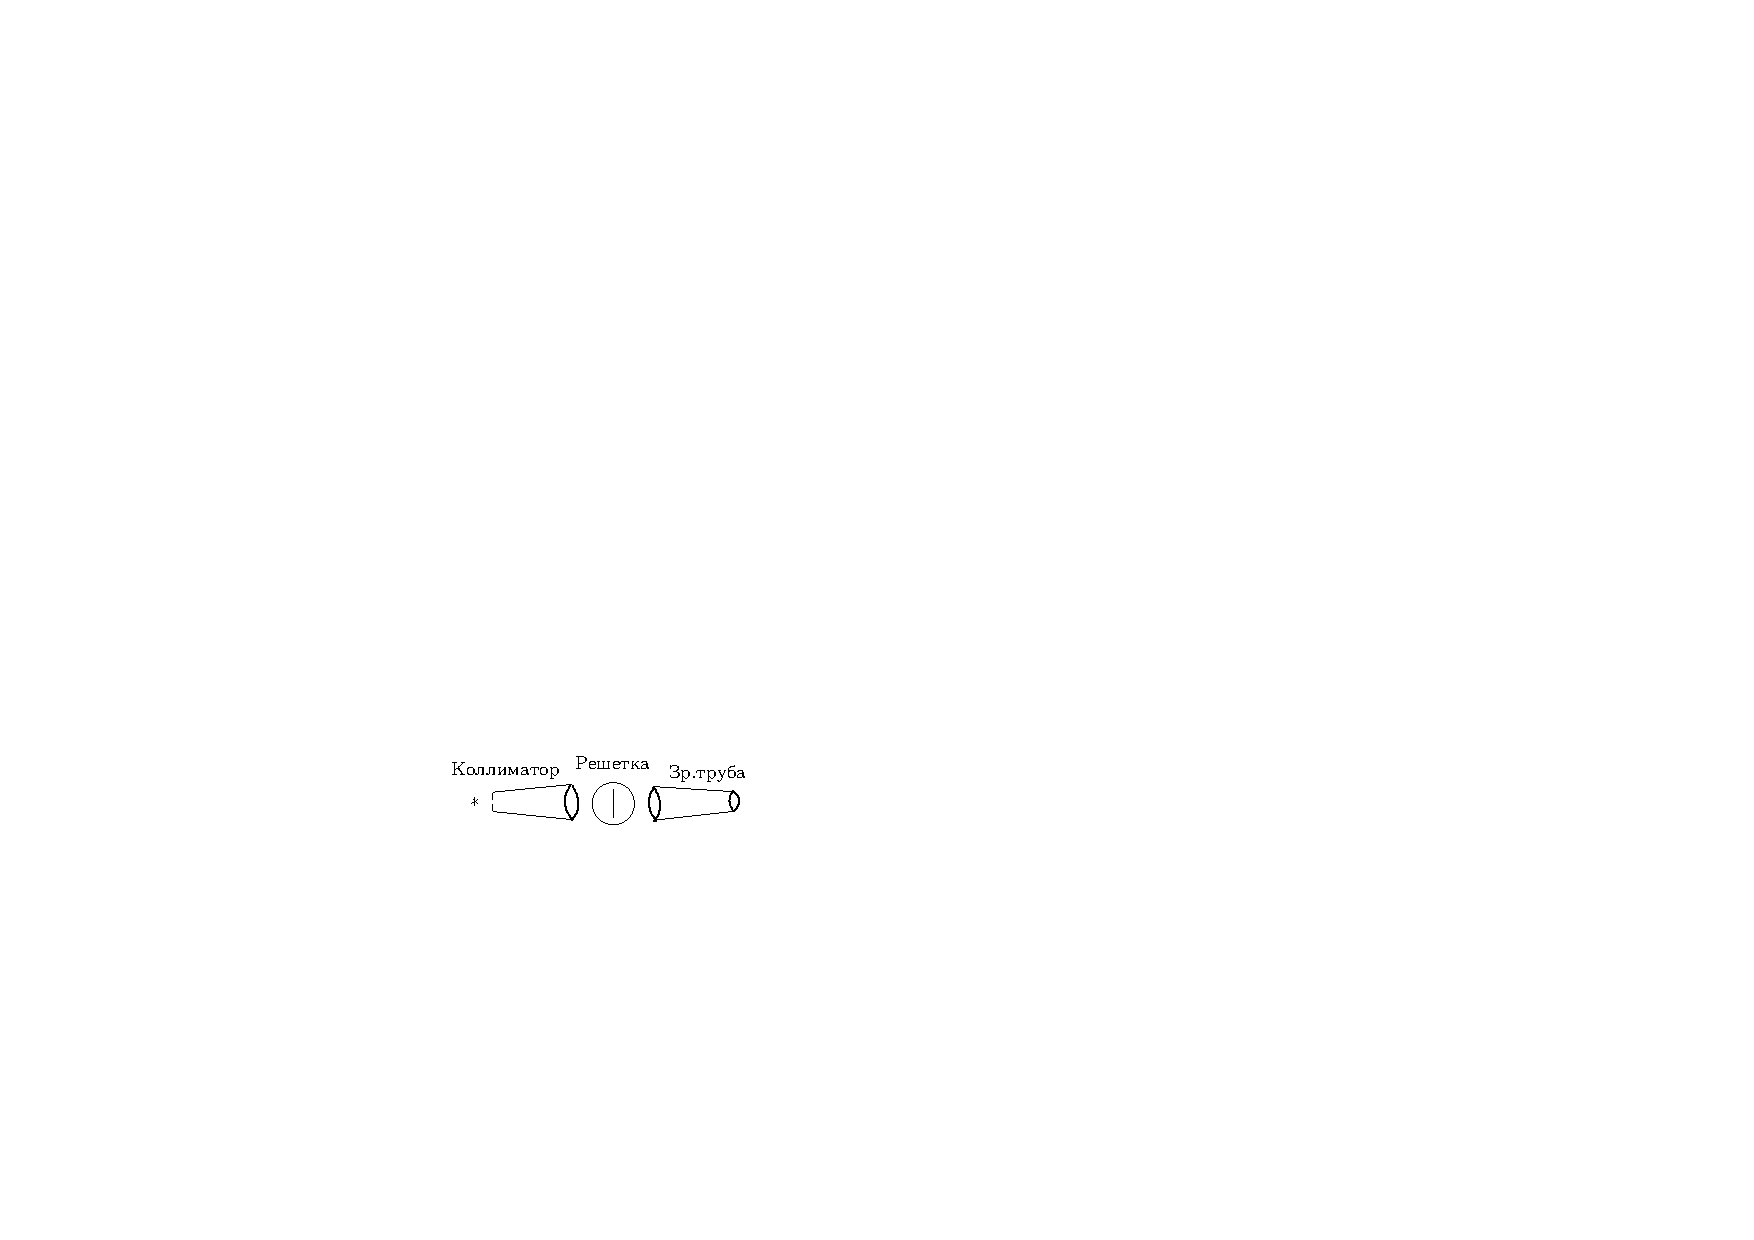
\includegraphics[scale=1.5]{inst}
	\caption{Схема установки.}
\end{figure}

\section{Обработка результатов}

	Запишем угловые координаты линий $\pm1$ порядка. Погрешность измерений составляет $5''$ или $2\cdot 10^{-5}$ рад. Поскольку невозможно точно настроиться на центр полосы.
	
	\begin{table}[H]
		\centering
		\begin{tabular}{|l|l|l|l|l|l|}
			\hline
			Цвет       & $\lambda$, нм & $\varphi_{+1}$, рад & $\varphi_{-1}$, рад & $\sin{\varphi_{+1}}$ & $\sin{\varphi_{-1}}$ \\ \hline
			красный    & -             & 0,31735             & -0,30785            & 0,31205              & -0,30301             \\ \hline
			красный    & -             & 0,31444             & -0,30495            & 0,30929              & -0,30024             \\ \hline
			желтый     & 579,1         & 0,29971             & -0,29037            & 0,29524              & -0,28631             \\ \hline
			желтый     & 577,0         & 0,29957             & -0,29029            & 0,29511              & -0,28623             \\ \hline
			зеленый    & 546,1         & 0,28217             & -0,27350            & 0,27844              & -0,27010             \\ \hline
			голубой    & 491,6         & 0,25310             & -0,24618            & 0,25041              & -0,24370             \\ \hline
			фиолетовый & 404,7         & 0,22399             & -0,21922            & 0,22212              & -0,21747             \\ \hline
		\end{tabular}
	\end{table}

	Погрешность синуса найдем следующим образом:
	\[
		\sigma_{\sin} = \sqrt{\left(\frac{\partial \sin\varphi}{\partial \varphi}\cdot\sigma_\varphi \right)^2} = |\cos\varphi\cdot\sigma_\varphi| \approx 2\cdot 10^{-5}
	\]
	
	Для линий спектра с известной длиной волны построим график зависимости $\sin{\varphi}$ от $\lambda$.
	
	\begin{figure}[H]
		\centering
		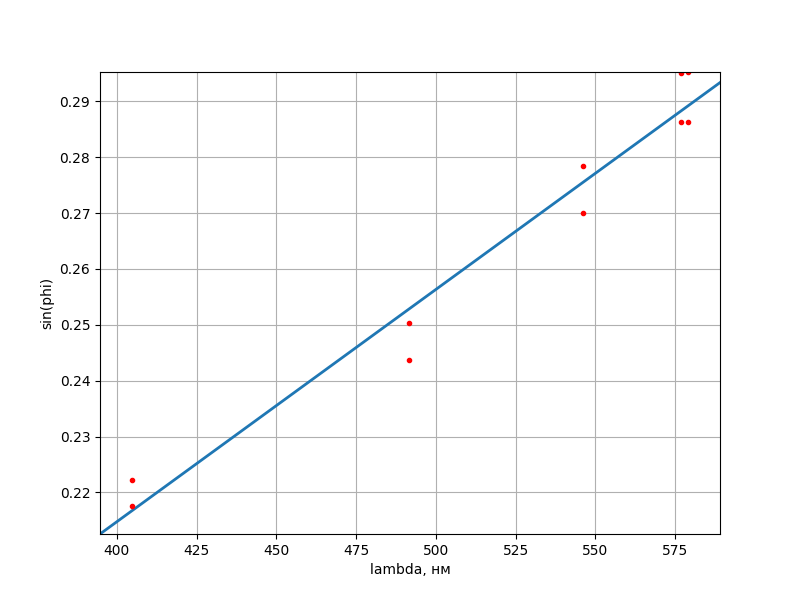
\includegraphics[scale=0.7]{gr1}
	\end{figure}

	Коэффициент наклона $k = (41\pm2)\cdot 10^{-5}$ нм$^{-1}$
	\[
		d= \frac{1}{k} = 2,43 \pm 0,11 \text{ мкм}
	\]
	\[
		\sigma_d = \frac{\sigma_k}{k^2}
	\]
	Значение шага, написанное на амплитудной решетке: $2$ мкм.
	
	Рассчитаем угловую дисперсию для спектров разного порядка. Для желтого дублета $\delta\lambda = 2,1$ нм.
	
	\begin{table}[H]
		\centering
		\begin{tabular}{|l|l|l|l|l|}
			\hline
			$m$ & $\varphi_{+1}$, рад & $\varphi_{-1}$, рад & $\delta\varphi$, рад & $D$, 1/нм \\ \hline
			-1  & -0,29009            & -0,29037            & 0,00028              & 0,00013   \\ \hline
			-2  & -0,59780            & -0,59949            & 0,00169              & 0,00080   \\ \hline
			+1  & 0,29957             & 0,29980             & 0,00023              & 0,00010   \\ \hline
			+2  & 0,64297             & 0,64586             & 0,00289              & 0,00137   \\ \hline
		\end{tabular}
	\end{table}
	\[
		\sigma_D = \frac{\sigma_{\delta\varphi}}{\delta\lambda} = 1\cdot 10^{-5} \text{ 1/нм}
	\]
	График зависимости угловой дисперсии от порядка спектра
	\begin{figure}[H]
		\centering
		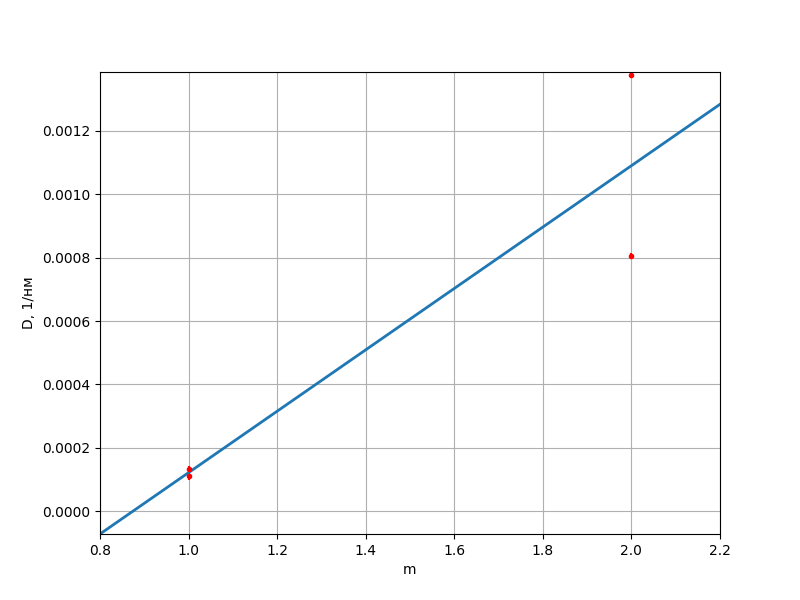
\includegraphics[scale=0.7]{gr2}
	\end{figure}

	Формула (2) дает значения для 1 порядка $D_1 = 5 \cdot 10^{-4}$ 1/нм, и для 2 порядка $D_2 \hm= 12 \cdot 10^{-4}$ 1/нм. Полученные значения совпадают по порядку.
	
	Оценим разрешимый спектральный интервал $\delta\lambda$
	\[
		\delta\lambda = \frac{\Delta\varphi}{D}
	\]
	\begin{table}[H]
		\centering
		\begin{tabular}{|l|l|l|l|l|}
			\hline
			$m$ & $\varphi_{+1}$, рад & $\varphi_{-1}$, рад & $\delta\varphi$, $10^{-5}$ рад & $\delta\lambda$, нм \\ \hline
			-1  & -0,29037            & -0,29038            & 1                              & 0,075               \\ \hline
			-2  & -0,59798            & -0,59796            & 2                              & 0,024               \\ \hline
			+1  & 0,30005             & 0,30004             & 1                              & 0,091               \\ \hline
			+2  & 0,64619             & 0,64616             & 3                              & 0,021               \\ \hline
		\end{tabular}
	\end{table}

	Усредняя получим
	\[
		\delta\lambda = 0,05\pm0,03 \text{ нм}
	\]
	Тогда, разрешающая способность 
	\[
		R = \frac{\lambda}{\delta\lambda} = 11000\pm7000
	\]
	
	Найдем число эффективно работающих штрихов $N = R/m$
	\begin{table}[H]
		\centering
		\begin{tabular}{|l|l|}
			\hline
			$m$ & $N$, $10^3$ \\ \hline
			1   & $11\pm7$    \\ \hline
			2   & $5\pm3$     \\ \hline
		\end{tabular}
	\end{table}

	Тогда эффективный размер решетки $l = Nd$:
	\begin{table}[H]
		\centering
		\begin{tabular}{|l|l|}
			\hline
			$m$ & $l$, мм   \\ \hline
			1   & $22\pm14$ \\ \hline
			2   & $11\pm7$  \\ \hline
		\end{tabular}
	\end{table}

	Можно оценить, что желтая линия наложится на фиолетовую при $m=6$ для желтого и $m =8$ для фиолетового. Поскольку
	\[
		0,29971\cdot6-0,22399\cdot8 = 0,00634
	\]
	
	\section{Вывод}
	В данной работе мы познакомились с устройством гониометра, а так же определили спектральные характеристики амплитудной решетки.
	
	

\end{document}
